\documentclass{article}
\usepackage{apacite}
\usepackage{hyperref}
\usepackage{multicol}
\usepackage{natbib}
\usepackage{andi}
\usepackage[utf8]{inputenc}
\usepackage{array}
\usepackage[first=0,last=9]{lcg}
\setlength{\parindent}{0pt}
\usepackage{hyperref}
\usepackage{pgfplots}
\usepgfplotslibrary{statistics}
\usepackage{physics}
\usepackage{soul}
\usepackage{tikz-cd}
\usepackage{courier} %% Sets font for listing as Courier.
\usepackage{listings, xcolor}
\usetikzlibrary{calc,patterns,angles,quotes}
\usepackage{pgfplots}
\pgfplotsset{width=15cm,height=10cm,compat=1.9}
\usepackage[english]{babel}
\usepackage{fancyhdr}
\usepackage{lastpage}
\pagestyle{empty}% for cropping
\usepackage{tikz}
\usepackage{tabu}
\newcounter{NoTableEntry}
\renewcommand*{\theNoTableEntry}{NTE-\the\value{NoTableEntry}}
\pagestyle{fancy}
\fancyhf{}
\cfoot{Page \thepage \hspace{1pt} of \pageref{LastPage}}
\usepackage{wrapfig}

    \lstset{
tabsize = 4, %% set tab space width
showstringspaces = false, %% prevent space marking in strings, string is defined as the text that is generally printed directly to the console
numbers = left, %% display line numbers on the left
commentstyle = \color{green}, %% set comment color
keywordstyle = \color{blue}, %% set keyword color
stringstyle = \color{red}, %% set string color
rulecolor = \color{black}, %% set frame color to avoid being affected by text color
basicstyle = \small \ttfamily , %% set listing font and size
breaklines = true, %% enable line breaking
numberstyle = \tiny,
}



\usepgfplotslibrary{external}


\newcommand{\boxplot}[6]{%
	%#1: center, #2: median, #3: 1/4 quartile, #4: 3/4 quartile, #5: min, #6: max
	\filldraw[fill=white,line width=0.2mm] let \n{boxxl}={#1-0.1}, \n{boxxr}={#1+0.1} in (axis cs:\n{boxxl},#3) rectangle (axis cs:\n{boxxr},#4);   % draw the box
	\draw[line width=0.2mm, color=red] let \n{boxxl}={#1-0.1}, \n{boxxr}={#1+0.1} in (axis cs:\n{boxxl},#2) -- (axis cs:\n{boxxr},#2);             % median
	\draw[line width=0.2mm] (axis cs:#1,#4) -- (axis cs:#1,#6);                                                                           % bar up
	\draw[line width=0.2mm] let \n{whiskerl}={#1-0.025}, \n{whiskerr}={#1+0.025} in (axis cs:\n{whiskerl},#6) -- (axis cs:\n{whiskerr},#6);        % upper quartile
	\draw[line width=0.2mm] (axis cs:#1,#3) -- (axis cs:#1,#5);                                                                           % bar down
	\draw[line width=0.2mm] let \n{whiskerl}={#1-0.025}, \n{whiskerr}={#1+0.025} in (axis cs:\n{whiskerl},#5) -- (axis cs:\n{whiskerr},#5);        % lower quartile
	}



%DowJones

\usepackage{pgfplots}
% Nice color sets, see see http://colorbrewer2.org/	
\usepgfplotslibrary{colorbrewer}
% initialize Set1-4 from colorbrewer (we're comparing 4 classes),
\pgfplotsset{compat = 1.15, cycle list/Set1-8} 
% Tikz is loaded automatically by pgfplots
\usetikzlibrary{pgfplots.statistics, pgfplots.colorbrewer} 
% provides \pgfplotstabletranspose
\usepackage{pgfplotstable}
\usepackage{filecontents}













\title{MDM4U1 Final Report}
\author{Andi Tse, Marven Wang, Michelle Zhou}
\date{June 9, 2023}
\rhead{Instructor: Ms. Hung}
\lhead{Andi Tse, Marven Wang, Michelle Zhou}
\chead{Final Report}
\rfoot{MDM4U1}
\lfoot{Data Management}

 


\begin{document}

\maketitle
\tableofcontents
\newpage



















\section{Introduction}
	This statistical study aims to reveal and compare the profitability of trading the ETFs of the three most popular indexes through the trends in the historical data. The following instruments and calculated indicators are used to display relevant patterns: short/long term SMA difference, slope of the EMA at different times, and two variable analyses between Relative Index and Average Price. The SMA difference and the EMA slope aims to show the growth pattern of the indexes as well as the amount of potential risk for investors. The Relative Index and Price analysis, on the other hand, helps label important support and resistance points. 
 \section{Terminologies and Explanations}
 To help better understand the study, here are some of the terminologies used and explanations needed to better understand the report.
\begin{enumerate}
    \item Day: unless otherwise specified, it means work days. A month is approximately 20 work days.
\item Indexes: they are the sum of a collection of stocks, which is usually too enormous in price to trade. This introduces the concept of index ETF. ETFs are managed such that their price very closely resembles the index price. Their volume represents a constant portion of the total trade activities around the index. 
\item Moving Average (MA): it is a value that is calculated at the same frequency of the price, they are generated by taking the average of the certain amount of past prices. The Simple Moving Average takes the arithmetic unweighted average, and Exponential Moving Average takes the average in a way such that the more recent price has exponentially more weight. The number behind represents the time period where the average is taken. For example, SMA10 means the simple moving average of the past 10 days. 
\item Relative Index (terminology varies per situation): in this case, it is the location of the daily average price relative to the price range of the day. It ranges from 0 (the average price being the lowest price) to 1 (the average price being the highest price). Its straightforward meaning is where the price “like” to stay in the range of oscillation of the day. Its trend when plotted against the price of the day indicates the growth potential of the index. 
\item Relationship between Relative Index and Price: it is first worth to note that the graph of the two variables is meant to have a medium strength. The reason being that only in the rarest situation is the period of one growth cycle precisely one day. This results in a deviation to the relationship between the two variables. The slope of the linear regression of the relationship, if positive, can show the power and potential of the current trend (how steady is the current trend and how much longer can it last). A non-positive slope indicates the imminent termination of the current trend or the continuation of a horizontal price movement.  

\end{enumerate}


\pagebreak
\section{Dow Jones Industrial Average (Marven)}


%include the data table here
\begin{align*}
    \text{Median }&=0.032     &        \sigma&=\sqrt{\frac{\sum\left(x_i-\mu\right)^2}{N}}\\
    Q1&=-1.4157     &  \sigma    &=\sqrt{\frac{\sum\left(x_i-\frac{1}{21}\sum x_i\right)^2}{21}}\\
    Q3&=1.072175 &        \sigma &=1.2683623513938
\end{align*}



\begin{figure}[h]
    \centering
    \begin{tikzpicture}
      \begin{axis}
        [
        xlabel={SMA Index (USD\$)},
        title=SMA 20-10 Difference Box and Whisker Plot for DIA,
        ytick={0},
        width = 1\textwidth,
        height = 0.15\textheight,
        enlarge y limits,
        xmin=-2.2,
        xmax=1.5,
       % xtick={-2,-1,0,1},
        boxplot/every median/.style={red, thick},
        extra x tick style={
           yshift=-15pt, % move them down a bit
           tickwidth=0 % and remove the ticks (small vertical lines)
           }
        ]
        \addplot[
            boxplot prepared={
              median= 0.032,
              lower quartile= -1.4157,
              upper quartile= 1.072175,
              lower whisker= -2.0775,
              upper whisker= 1.38765
            },
            ] coordinates {};
    \end{axis}
\end{tikzpicture}
\end{figure}

The median of the SMA difference over the 20 day interval is slightly positive, but the location of Q1 and Q3 indicates that the data is almost evenly spread out on both sides of the zero line. This means that the price is in the state of horizontal movement in the grand scope of 40-60 days (2 to 3 months). The standard deviation of the data set means that there are significant oscillations in the same scope of time. The reason behind this conclusion from a seemingly small deviation is that for the difference of SMAs to be \_ dollars, the price must vary in 5-10 times of that amount.
%include data table
\begin{align*}
    \text{Median }&=0.36735351565        &    Q1&=-0.4256513672\\
    \sigma&=0.93318408045431        &  Q3&=0.97270996095
\end{align*}


\begin{figure}[h]
    \centering
    \begin{tikzpicture}
      \begin{axis}
        [
        xlabel={EMA Slope (USD\$/day)},
        title=EMA Slope Box and Whisker Plot for DIA,
        ytick={0},
        width = 1\textwidth,
        height = 0.15\textheight,
        enlarge y limits,
        xmin=-1.5,
        xmax=3,
       % xtick={-2,-1,0,1},
        boxplot/every median/.style={red, thick},
        extra x tick style={
           yshift=-15pt, % move them down a bit
           tickwidth=0 % and remove the ticks (small vertical lines)
           }
        ]
        %    \addplot coordinates{(2.1889,0)} node[right,font=\scriptsize] at (boxplot box cs: \boxplotvalue{average}, 0.95)
    {\boxplotvalue{average}}; 
        \addplot[
            boxplot prepared={
              median= 0.36735351565,
              lower quartile= -0.4256513672,
              upper quartile= 0.97270996095,
              lower whisker= -1.315726563,
              upper whisker= 2.747210938
              %2.1889
            },
            ] coordinates {};

            %\addplot[color=black,mark=square,]coordinates{(2.1889,1)};
    \end{axis}
\end{tikzpicture}
\end{figure}
The median, Q3, and the maximum all lean toward the positive side compared to Q1 and the minimum. This means that there exists a growth pattern in the short term, with a scope of 10-20 days. The fact that the whisker reaches far into the negative region indicates a relatively high risk of the pattern terminating suddenly. This aligns with the previous conclusion since there is no long-term trend established.



%include data table
\begin{align*}
    a&=\frac{n \sum x y-\left(\sum x\right)\left(\sum y\right)}{n\left(\sum x^2\right)-\left(\sum x\right)^2} & b&=\bar{y}-a \bar{x} & r&=\frac{n \sum x y-\left(\sum x\right)\left(\sum y\right)}{\sqrt{\left[n \sum x^2-\left(\sum x\right)^2\right]\left[n \sum y^2-\left(\sum y\right)^2\right]}}\\
    a&=5.82     & b&=172         & r&=0.3991
\end{align*}

\begin{center}
\begin{tikzpicture}
\begin{axis}[
    enlargelimits=false,
    title={DowJones WAP vs. Relative Index},
    xlabel={Relative Index},
    ylabel={WAP},
    xmin=0.2, xmax=0.8,
    ymin=165, ymax=185,
%    xtick={0,0.1,0.2,0.3,0.4,0.5,0.6},
%    ytick={-4,-3,-2,-1,0,1,2},
    legend pos=south east,
    ymajorgrids=true,
    xmajorgrids=true,
    grid style=dashed,
]
\addplot[
    color=blue,
    only marks,
    mark=square,]
table[meta=R.I]
{DowJones_WAP vs Relative Index.dat};



\addplot [
    domain=0:0.8, 
    samples=100, 
    color=blue,
    ]
{5.82*x+172};
\addlegendentry{\(5.82x+172\)}

\end{axis}
\end{tikzpicture}
\end{center}


The plot of relative index against the weighted price displays a positive slope of \_, which indicates that the price tends to be higher at higher relative index. This means that the price is likely to follow the growth trend demonstrated by the EMA slope chart and change the long-term state from horizontal movement to a net growth. The coefficient of correlation is \_ . Although it is meaningless on its own (using a time period that is not matched with the growth period), it can be compared with the other indexes to show a relative uncertainty of this conclusion.


\pagebreak
\section{Russell 2000 Index (Michelle)}

%include the data table here
\begin{align*}
    \text{Median }&=-3.8108     &        \sigma&=\sqrt{\frac{\sum\left(x_i-\mu\right)^2}{N}}\\
    Q1&=-5.63915     &  \sigma    &=\sqrt{\frac{\sum\left(x_i-\frac{1}{21}\sum x_i\right)^2}{21}}\\
    Q3&=-2.03875 &        \sigma &=1.7697509067137
\end{align*}

\begin{figure}[h]
    \centering
    \begin{tikzpicture}
      \begin{axis}
        [
        xlabel={SMA Index (USD\$)},
        title=SMA 20-10 Difference Box and Whisker Plot for IWM,
        ytick={0},
        width = 1\textwidth,
        height = 0.15\textheight,
        enlarge y limits,
        xmin=-7,
        xmax=-1,
       % xtick={-2,-1,0,1},
        boxplot/every median/.style={red, thick},
        extra x tick style={
           yshift=-15pt, % move them down a bit
           tickwidth=0 % and remove the ticks (small vertical lines)
           }
        ]
        \addplot[
            boxplot prepared={
              median= -3.8108,
              lower quartile= -5.63915,
              upper quartile= -2.03875,
              lower whisker= -6.70415,
              upper whisker= -1.5
            },
            ] coordinates {};
    \end{axis}
\end{tikzpicture}
\end{figure}

The median of the SMA difference over the 20 day interval is negative, the location of Q1 and Q3 indicates that the data is skewed heavily towards the negative and does not have a zero line present within the graph. This observation shows that the price is in a state of horizontal movement in the grand scope of 2-3 months. The standard deviation in the graph reveals the data is more or less stable without major changes due to it staying mostly within the negative range. The reasoning behind this conclusion is simple: the difference of SMA to be  dollars, the price must vary 5-10 times of the amount.

%include data table
\begin{align*}
    \text{Median }&= -0.21594628905        &    Q1&=-1.753652832\\
    \sigma&=1.5760721799391        &  Q3&=0.7495527344
\end{align*}


\begin{figure}[h]
    \centering
    \begin{tikzpicture}
      \begin{axis}
        [
        xlabel={EMA Slope (USD\$/day)},
        title=EMA Slope Box and Whisker Plot for IWM,
        ytick={0},
        width = 1\textwidth,
        height = 0.15\textheight,
        enlarge y limits,
        xmin=-4.5,
        xmax=2,
       % xtick={-2,-1,0,1},
        boxplot/every median/.style={red, thick},
        extra x tick style={
           yshift=-15pt, % move them down a bit
           tickwidth=0 % and remove the ticks (small vertical lines)
           }
        ]
        %    \addplot coordinates{(2.1889,0)} node[right,font=\scriptsize] at (boxplot box cs: \boxplotvalue{average}, 0.95)
    {\boxplotvalue{average}}; 
        \addplot[
            boxplot prepared={
              median= -0.21594628905,
              lower quartile= -1.753652832,
              upper quartile= 0.7495527344,
              lower whisker= -4.151644531,
              upper whisker= 1.566734375
              %2.1889
            },
            ] coordinates {};

            %\addplot[color=black,mark=square,]coordinates{(2.1889,1)};
    \end{axis}
\end{tikzpicture}
\end{figure}
The median, Q3, and the maximum for Russel all lean toward the negative. Within a scope of 10-20 days, there exists only a decay pattern. Since the range of the whisker stays firmly within the negatives, there is little risk of the pattern terminating without an extreme amount of outliers being inputted into the data. 



%include data table
\begin{align*}
    a&=\frac{n \sum x y-\left(\sum x\right)\left(\sum y\right)}{n\left(\sum x^2\right)-\left(\sum x\right)^2} & b&=\bar{y}-a \bar{x} & r&=\frac{n \sum x y-\left(\sum x\right)\left(\sum y\right)}{\sqrt{\left[n \sum x^2-\left(\sum x\right)^2\right]\left[n \sum y^2-\left(\sum y\right)^2\right]}}\\
    a&=-2.18     & b&=178         & r&=0.0642
\end{align*}


\begin{center}
\begin{tikzpicture}
\begin{axis}[
    enlargelimits=false,
    title={Russell WAP vs. Relative Index},
    xlabel={Relative Index},
    ylabel={WAP},
    xmin=0, xmax=0.8,
    ymin=160, ymax=200,
%    xtick={0,0.1,0.2,0.3,0.4,0.5,0.6},
%    ytick={-4,-3,-2,-1,0,1,2},
    legend pos=south east,
    ymajorgrids=true,
    xmajorgrids=true,
    grid style=dashed,
]
\addplot[
    color=blue,
    only marks,
    mark=square,]
table[meta=R.I]
{Russell_WAP vs Relative Index.dat};



\addplot [
    domain=0:0.8, 
    samples=100, 
    color=blue,
    ]
{-2.18*x+178};
\addlegendentry{\(-2.18x+178\)}

\end{axis}
\end{tikzpicture}
\end{center}
The plot of the relative index against the weighted price displays a negative slope of  , which indicates that the price tends to be lower at higher relative index. This shows that the price is likely to follow the decay trend demonstrated in the EMA slope chart and change the long-term state from horizontal movement to net growth. The coefficient of correlation is . It can be compared with the other indexes to show a relative uncertainty of this conclusion.


\pagebreak
\section{SPDR S\&P 500 ETF Trust (Andi)}

%include the data table here
\begin{align*}
    \text{Median }&=-3.36305    &        \sigma&=\sqrt{\frac{\sum\left(x_i-\mu\right)^2}{N}}\\
    Q1&=-4.13835     &  \sigma    &=\sqrt{\frac{\sum\left(x_i-\frac{1}{21}\sum x_i\right)^2}{21}}\\
    Q3&=-2.039325 &        \sigma &=2.0230822611682
\end{align*}

\begin{figure}[h]
    \centering
    \begin{tikzpicture}
      \begin{axis}
        [
        xlabel={SMA Index (USD\$)},
        title=SMA 20-10 Difference Box and Whisker Plot for SPY,
        ytick={0},
        width = 1\textwidth,
        height = 0.15\textheight,
        enlarge y limits,
        xmin=-6.5,
        xmax=2.5,
       % xtick={-2,-1,0,1},
        boxplot/every median/.style={red, thick},
        extra x tick style={
           yshift=-15pt, % move them down a bit
           tickwidth=0 % and remove the ticks (small vertical lines)
           }
        ]
        %    \addplot coordinates{(2.1889,0)} node[right,font=\scriptsize] at (boxplot box cs: \boxplotvalue{average}, 0.95)
    {\boxplotvalue{average}}; 
        \addplot[
            boxplot prepared={
              median= -3.36305,
              lower quartile= -4.13835,
              upper quartile= -2.039325,
              lower whisker= -6.0179,
              upper whisker= 0.78355
              %2.1889
            },
            ] coordinates {};

            \addplot[color=black,mark=square,]coordinates{(2.1889,1)};
    \end{axis}
\end{tikzpicture}
\end{figure}

The median of the SMA difference over the 20 day interval is slightly positive. The location of Q1 and Q3 indicates that the data is almost evenly spread out on both sides of the zero line. This means that the price is in the state of horizontal movement in the grand scope of 40-60 days. The standard deviation of the data set means that there are significant oscillations in the same scope of time. The reason behind this conclusion is from a seemingly small deviation. For the difference of SMAs to be   dollars, the price must vary in 5-10 times of that amount.



%include data table
\begin{align*}
    \text{Median }&=0.314605468735        &    Q1&=-1.43592675775\\
    \sigma&=2.2372048153341        &  Q3&=2.38305712875
\end{align*}






\begin{figure}[h]
    \centering
    \begin{tikzpicture}
      \begin{axis}
        [
        xlabel={EMA Slope (USD\$/day)},
        title=EMA Slope Box and Whisker Plot for SPY,
        ytick={0},
        width = 1\textwidth,
        height = 0.15\textheight,
        enlarge y limits,
        xmin=-5,
        xmax=3.7,
       % xtick={-2,-1,0,1},
        boxplot/every median/.style={red, thick},
        extra x tick style={
           yshift=-15pt, % move them down a bit
           tickwidth=0 % and remove the ticks (small vertical lines)
           }
        ]
        %    \addplot coordinates{(2.1889,0)} node[right,font=\scriptsize] at (boxplot box cs: \boxplotvalue{average}, 0.95)
    {\boxplotvalue{average}}; 
        \addplot[
            boxplot prepared={
              median= 0.314605468735,
              lower quartile= -1.43592675775,
              upper quartile= 2.38305712875,
              lower whisker= -4.611535156,
              upper whisker= 3.462884766
              %2.1889
            },
            ] coordinates {};

            %\addplot[color=black,mark=square,]coordinates{(2.1889,1)};
    \end{axis}
\end{tikzpicture}
\end{figure}

The median, Q3, and the maximum all lean toward the positive side compared to Q1 and the minimum. This means that there exists a growth pattern in the short term with a scope of 10-20 days. The fact that the whisker reaches into the deeper parts of the negative region indicates that there is a high risk of the pattern termination suddenly. This aligns with the previous conclusion since there is no long-term trend established.



%include data table
\begin{align*}
    a&=\frac{n \sum x y-\left(\sum x\right)\left(\sum y\right)}{n\left(\sum x^2\right)-\left(\sum x\right)^2} & b&=\bar{y}-a \bar{x} & r&=\frac{n \sum x y-\left(\sum x\right)\left(\sum y\right)}{\sqrt{\left[n \sum x^2-\left(\sum x\right)^2\right]\left[n \sum y^2-\left(\sum y\right)^2\right]}}\\
    a&=11     & b&=390         & r&=0.2566
\end{align*}

\begin{center}
\begin{tikzpicture}
\begin{axis}[
    enlargelimits=false,
    title={SPY WAP vs. Relative Index},
    xlabel={Relative Index},
    ylabel={WAP},
    xmin=0.2, xmax=0.9,
    ymin=370, ymax=420,
%    xtick={0,0.1,0.2,0.3,0.4,0.5,0.6},
%    ytick={-4,-3,-2,-1,0,1,2},
    legend pos=south east,
    ymajorgrids=true,
    xmajorgrids=true,
    grid style=dashed,
]
\addplot[
    color=blue,
    only marks,
    mark=square,]
table[meta=R.I]
{SPY_WAP vs Relative Index.dat};



\addplot [
    domain=0:1, 
    samples=100, 
    color=blue,
    ]
{11*x+390};
\addlegendentry{\(11x+390\)}

\end{axis}
\end{tikzpicture}
\end{center}

The plot of relative index against the weighted price displays a positive slope of   , which indicates that the price tends to be higher at higher relative index. This means that the price is likely to follow the growth trend demonstrated by the EMA slope chart and change the long-term state from horizontal movement to net growth. The coefficient of correlation is    . Although it is meaningless on its own, it can be compared to the other indexes to show a relative uncertainty of this conclusion.






\pagebreak
\section{Conclusion}
To sum up, the analysis of the three index ETFs are: \\
DIA only displays a growth pattern in the short term, but the relative index indicates that the short term trend has the potential of becoming the new long term trend. IWM is currently in a long term descending trend that is predicted to end, followed by horizontal movements. SPY is in a long term descending trend that is predicted to last for a long period of time. 

\subsection{Investment Strategy - Short Serm}
The optimum strategy around the three ETFs in the scope of 20 days is to buy DIA with $60\%$ of the available fund at a local low point and sell when it reaches a relative high point in the past month. The rest of the fund can be used in shorting SPY, but it should be done in a cautious way such that the position should be closed when the price demonstrates a slight growth pattern.
\subsection{Investment Strategy - Long Term}
The optimum investment strategy in the scope of 40 days is to short SPY with most of the funds. For this strategy, the investor can be more lenient on closing their positions over a small rebounce, the reason being that the relative index demonstrates a great trend-sustaining potential. The remaining funds should be invested in DIA if future price movements support the assumption that the short term growth pattern will become the long term pattern. The reason to put a small quantity of the fund into buying DIA is because of the fact that the SMA difference statistics does not yet support a long-term growth pattern.


\section{Risk Analysis}
\begin{comment}
For the short term strategy, the risk is $____$, supported by the standard deviation of the EMA slope. The standard deviation of the SMA difference and EMA slope data sets are relatively _____, as calculated previously. This implies that there is a relatively ___ chance of the price not behaving as predicted by the central tendency of the data.\\
For the long term strategy, the risk is _____. Compare the coefficient of correlation of the three relative index plots, it is noted that the coefficient for SPY is the _____ out of the three. This means that even though the data period is out of phase, it can still be concluded that the uncertainty of this analysis for SPY is the ____. To conclude, the best strategy that can be derived from this research have a _____ risk involved when executing
\end{comment}

\end{document}